% =====================================================================
% FIGURE 2 — the two architectural modifications.
% Layout convention: the VERTICAL axis is the pyramid level (P5/32 at the
% top, P2/4 at the bottom) and the HORIZONTAL axis is depth through the
% network. Every edge is transcribed from the `from` field of the YAML;
% Conv-downsample and Concat rows are folded into the edge LABELS so that
% only tensor-producing blocks appear as boxes.
%
%   (a) BACKBONE + HEAD_DYSAMPLE + TAIL_LS_SHIFT  (run_arch_port_v6i.py)
%       9<-8  11<-[9,6]  12<-11  14<-[12,4]  17<-[15,11]  20<-[19,8]
%       21<-14  23<-[21,2]  24<-23  25<-14  26<-17  27<-20  28<-[24..27]
%   (b) yolo26-p2dys-p234rich.yaml
%       13<-[11,6]  16<-[14,4]  17<-16  19<-[17,2]  22<-[20,16]
%       25<-[23,13]  26<-[19,22,25]
% =====================================================================
\begin{figure*}[t]
\centering
\iffigpng
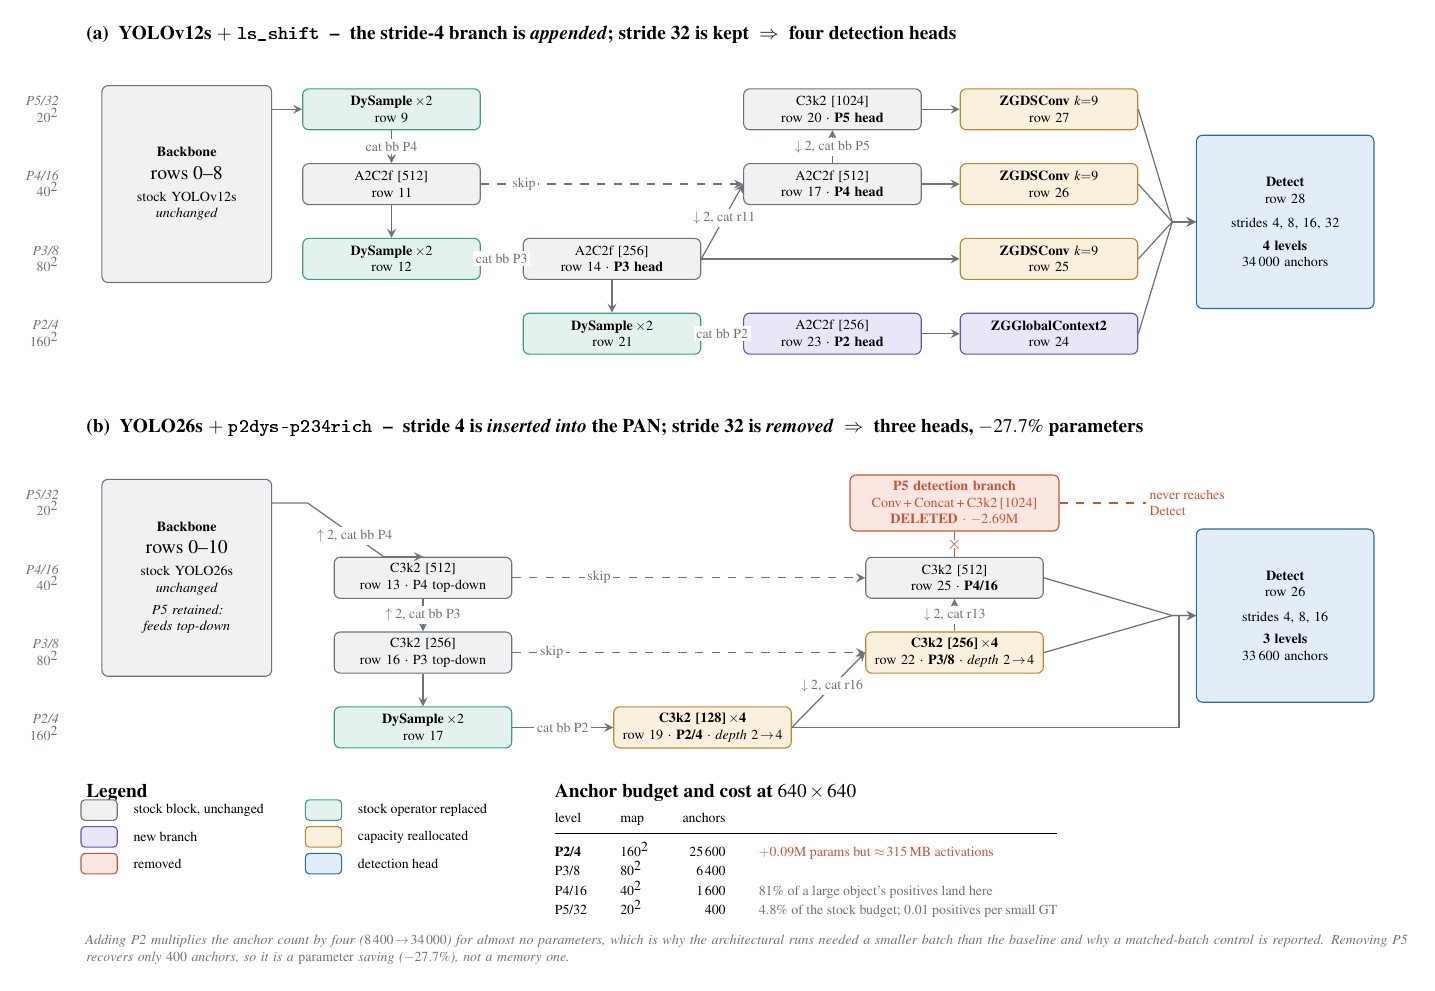
\includegraphics[width=\linewidth]{fig2.png}
\else
\begin{tikzpicture}[x=1cm,y=1cm,
  nd/.style={blk,minimum height=5.2mm,inner sep=2.2pt,font=\tiny,text width=21mm},
  hd/.style={font=\scriptsize\bfseries,align=left},
  el/.style={font=\tiny,text=cGry,fill=white,inner sep=1pt},
  lv/.style={font=\tiny\itshape,text=cGry,anchor=east,align=right},
  strk/.style={nd,draw=cCor,fill=cCorBg,text=cCor},
]
\def\LV{-0.60} \def\LIV{-1.55} \def\LIII{-2.50} \def\LII{-3.45}

% =====================================================================
% (a) YOLOv12s + ls_shift
% =====================================================================
\node[hd,anchor=west] at (0.15,0.35) {(a)~~YOLOv12s\;$+$\;\texttt{ls\_shift} \;--\; the stride-4 branch is \emph{appended}; stride 32 is kept \;$\Rightarrow$\; four detection heads};

\node[lv] at (0.05,\LV)   {P5/32\\$20^2$};  \node[lv] at (0.05,\LIV) {P4/16\\$40^2$};
\node[lv] at (0.05,\LIII) {P3/8\\$80^2$};   \node[lv] at (0.05,\LII) {P2/4\\$160^2$};

\node[nd,fill=cGryBg,draw=cGry,minimum height=25mm,text width=20mm] (a_bb) at (1.55,\LIV)
  {\textbf{Backbone}\\\scriptsize rows 0--8\\[2pt]\tiny stock YOLOv12s\\\tiny\emph{unchanged}};

\node[nd,draw=cTeal,fill=cTealBg] (a9)  at (4.15,\LV)   {\textbf{DySample}\,$\times2$\\\tiny row 9};
\node[nd]                          (a11) at (4.15,\LIV)  {A2C2f [512]\\\tiny row 11};
\node[nd,draw=cTeal,fill=cTealBg] (a12) at (4.15,\LIII) {\textbf{DySample}\,$\times2$\\\tiny row 12};

\node[nd]                          (a14) at (6.95,\LIII) {A2C2f [256]\\\tiny row 14 · \textbf{P3 head}};
\node[nd,draw=cTeal,fill=cTealBg] (a21) at (6.95,\LII)  {\textbf{DySample}\,$\times2$\\\tiny row 21};

\node[nd]                          (a20) at (9.75,\LV)   {C3k2 [1024]\\\tiny row 20 · \textbf{P5 head}};
\node[nd]                          (a17) at (9.75,\LIV)  {A2C2f [512]\\\tiny row 17 · \textbf{P4 head}};
\node[nd,draw=cPurp,fill=cPurpBg] (a23) at (9.75,\LII)  {A2C2f [256]\\\tiny row 23 · \textbf{P2 head}};

\node[nd,draw=cAmb,fill=cAmbBg]   (a27) at (12.5,\LV)   {\textbf{ZGDSConv} $k{=}9$\\\tiny row 27};
\node[nd,draw=cAmb,fill=cAmbBg]   (a26) at (12.5,\LIV)  {\textbf{ZGDSConv} $k{=}9$\\\tiny row 26};
\node[nd,draw=cAmb,fill=cAmbBg]   (a25) at (12.5,\LIII) {\textbf{ZGDSConv} $k{=}9$\\\tiny row 25};
\node[nd,draw=cPurp,fill=cPurpBg] (a24) at (12.5,\LII)  {\textbf{ZGGlobalContext2}\\\tiny row 24};

\node[nd,draw=cBlu,fill=cBluBg,minimum height=22mm,text width=21mm] (adet) at (15.5,\LIII+0.47)
  {\textbf{Detect}\\\tiny row 28\\[3pt]\tiny strides 4, 8, 16, 32\\[2pt]\tiny\textbf{4 levels}\\\tiny 34\,000 anchors};

% --- true edges ---
\draw[fl] (a_bb.east|-a9) -- (a9.west);
\draw[fl] (a9.south)  -- node[el]{cat bb P4} (a11.north);
\draw[fl] (a11.south) -- (a12.north);
\draw[fl] (a12.east)  -- node[el]{cat bb P3} (a14.west);
\draw[fl] (a14.east)  -- node[el,pos=0.55]{$\downarrow2$, cat r11} (a17.west);
\draw[fl] (a17.north) -- node[el]{$\downarrow2$, cat bb P5} (a20.south);
\draw[fl] (a14.south) -- (a21.north);
\draw[fl] (a21.east)  -- node[el]{cat bb P2} (a23.west);
\draw[flb] (a11.east) -- ++(0.55,0) |- node[el,pos=0.28]{skip} (a17.west);
\draw[fl] (a20.east) -- (a27.west);
\draw[fl] (a17.east) -- (a26.west);
\draw[fl] (a14.east) -- ++(0.35,0) -- ($(a25.west)+(-0.35,0)$) -- (a25.west);
\draw[fl] (a23.east) -- (a24.west);
\foreach \s in {a24,a25,a26,a27} \draw[fl] (\s.east) -- ($(adet.west)+(-0.3,0)$) -- (adet.west);

% =====================================================================
% (b) YOLO26s + p2dys-p234rich
% =====================================================================
\begin{scope}[yshift=-5.0cm]
\node[hd,anchor=west] at (0.15,0.35) {(b)~~YOLO26s\;$+$\;\texttt{p2dys-p234rich} \;--\; stride 4 is \emph{inserted into} the PAN; stride 32 is \emph{removed} \;$\Rightarrow$\; three heads, $-27.7\%$ parameters};

\node[lv] at (0.05,\LV)   {P5/32\\$20^2$};  \node[lv] at (0.05,\LIV) {P4/16\\$40^2$};
\node[lv] at (0.05,\LIII) {P3/8\\$80^2$};   \node[lv] at (0.05,\LII) {P2/4\\$160^2$};

\node[nd,fill=cGryBg,draw=cGry,minimum height=25mm,text width=20mm] (b_bb) at (1.55,\LIV)
  {\textbf{Backbone}\\\scriptsize rows 0--10\\[2pt]\tiny stock YOLO26s\\\tiny\emph{unchanged}\\[2pt]\tiny\emph{P5 retained:}\\\tiny\emph{feeds top-down}};

\node[nd]                          (b13) at (4.55,\LIV)  {C3k2 [512]\\\tiny row 13 · P4 top-down};
\node[nd]                          (b16) at (4.55,\LIII) {C3k2 [256]\\\tiny row 16 · P3 top-down};
\node[nd,draw=cTeal,fill=cTealBg] (b17) at (4.55,\LII)  {\textbf{DySample}\,$\times2$\\\tiny row 17};

\node[nd,draw=cAmb,fill=cAmbBg]   (b19) at (8.10,\LII)  {\textbf{C3k2 [128]}\,$\times\mathbf{4}$\\\tiny row 19 · \textbf{P2/4} · \emph{depth $2\!\to\!4$}};
\node[nd,draw=cAmb,fill=cAmbBg]   (b22) at (11.3,\LIII) {\textbf{C3k2 [256]}\,$\times\mathbf{4}$\\\tiny row 22 · \textbf{P3/8} · \emph{depth $2\!\to\!4$}};
\node[nd]                          (b25) at (11.3,\LIV)  {C3k2 [512]\\\tiny row 25 · \textbf{P4/16}};

\node[strk,text width=25mm]        (b5x) at (11.3,\LV)   {\textbf{P5 detection branch}\\\tiny Conv\,+\,Concat\,+\,C3k2\,[1024]\\\tiny\textbf{DELETED} · $-2.69$M};

\node[nd,draw=cBlu,fill=cBluBg,minimum height=22mm,text width=21mm] (bdet) at (15.5,\LIII+0.47)
  {\textbf{Detect}\\\tiny row 26\\[3pt]\tiny strides 4, 8, 16\\[2pt]\tiny\textbf{3 levels}\\\tiny 33\,600 anchors};

% --- true edges ---
% main path. NOTE: row 11 upsamples the BACKBONE P5 output (row 10), so this
% edge must leave the backbone at the P5 line, not at P4.
\draw[fl] (b_bb.east|-0,\LV) -- ++(0.45,0) -- node[el,pos=0.62]{$\uparrow2$, cat bb P4} ($(b13.north)+(-0.5,0)$) -- ($(b13.north)+(-0.5,0)$) -- (b13.north);
\draw[fl] (b13.south) -- node[el]{$\uparrow2$, cat bb P3} (b16.north);
\draw[fl] (b16.south) -- (b17.north);
\draw[fl] (b17.east)  -- node[el]{cat bb P2} (b19.west);
\draw[fl] (b19.east)  -- node[el,pos=0.55]{$\downarrow2$, cat r16} (b22.west);
\draw[fl] (b22.north) -- node[el]{$\downarrow2$, cat r13} (b25.south);
\draw[flb] (b16.east) -- ++(0.5,0) |- node[el,pos=0.3]{skip} (b22.west);
\draw[flb] (b13.east) -- ++(1.1,0) |- node[el,pos=0.3]{skip} (b25.west);
% row 19 routes BELOW rows 22/25 rather than clipping their labels
\draw[fl] (b19.east) -- ++(0.3,0) -- (14.15,\LII) -- (14.15,\LIII+0.47) -- (bdet.west);
\foreach \s in {b22,b25} \draw[fl] (\s.east) -- ($(bdet.west)+(-0.3,0)$) -- (bdet.west);
% the deleted branch, shown hanging off the P4 head where it used to attach
\draw[dashed,draw=cCor,line width=0.5pt] (b25.north) -- (b5x.south);
\node[text=cCor,font=\scriptsize\bfseries] at ($(b25.north)!0.5!(b5x.south)$) {$\times$};
\draw[dashed,draw=cCor,line width=0.5pt] (b5x.east) -- ++(1.1,0)
  node[el,text=cCor,right=0pt,align=left]{never reaches\\Detect};
\end{scope}

% =====================================================================
% (c) legend + the per-level budget that makes the cost visible
% =====================================================================
\begin{scope}[yshift=-9.05cm]
\node[anchor=north west,font=\scriptsize\bfseries] at (0.15,0) {Legend};
% swatches drawn as plain nodes: a tabular of nested \tikz pictures does not
% survive inside a tikz node, so the two columns are placed explicitly.
\foreach \i/\col/\bg/\txt in {0/cGry/cGryBg/{stock block, unchanged},
                              1/cPurp/cPurpBg/{new branch},
                              2/cCor/cCorBg/{removed}}{
  \node[draw=\col,fill=\bg,rounded corners=1.4pt,minimum width=4.6mm,minimum height=2.6mm,
        inner sep=0pt,anchor=west] at (0.20,-0.45-0.34*\i) {};
  \node[anchor=west,font=\tiny] at (0.75,-0.45-0.34*\i) {\txt};
}
\foreach \i/\col/\bg/\txt in {0/cTeal/cTealBg/{stock operator replaced},
                              1/cAmb/cAmbBg/{capacity reallocated},
                              2/cBlu/cBluBg/{detection head}}{
  \node[draw=\col,fill=\bg,rounded corners=1.4pt,minimum width=4.6mm,minimum height=2.6mm,
        inner sep=0pt,anchor=west] at (3.05,-0.45-0.34*\i) {};
  \node[anchor=west,font=\tiny] at (3.60,-0.45-0.34*\i) {\txt};
}

\node[anchor=north west,font=\scriptsize\bfseries] at (6.1,0) {Anchor budget and cost at $640\times640$};
\node[anchor=north west,font=\tiny] at (6.1,-0.34) {%
\begin{tabular}{@{}llrl@{}}
level & map & anchors & \\
\midrule
\textbf{P2/4}  & $160^2$ & $25\,600$ & \textcolor{cCor}{$+0.09$M params but $\approx\!315$\,MB activations} \\
P3/8           & $80^2$  & $6\,400$  & \\
P4/16          & $40^2$  & $1\,600$  & \textcolor{cGry}{$81\%$ of a large object's positives land here} \\
P5/32          & $20^2$  & $400$     & \textcolor{cGry}{$4.8\%$ of the stock budget; $0.01$ positives per small GT} \\
\end{tabular}};

\node[anchor=north west,font=\tiny\itshape,text=cGry,text width=168mm,align=left] at (0.15,-1.92)
 {Adding P2 multiplies the anchor count by four ($8\,400\!\to\!34\,000$) for almost no parameters, which is why the architectural runs
  needed a smaller batch than the baseline and why a matched-batch control is reported. Removing P5 recovers only $400$ anchors, so it is
  a \emph{parameter} saving ($-27.7\%$), not a memory one.};
\end{scope}

\end{tikzpicture}
\fi
\caption{The two architectural modifications. The vertical axis is the pyramid level and the horizontal axis is depth through the network; solid arrows are
the main data path, dashed arrows are lateral skips, and \texttt{Conv}-downsample and \texttt{Concat} rows are folded into the edge labels so that only
tensor-producing blocks are drawn. (a)~On YOLOv12s the stride-4 branch is \emph{appended}: the existing top-down/bottom-up path (rows 9--20) is left intact, a
P2 head is built from row 14 by content-aware upsampling, and each of the four levels then receives one gated refinement block --- global context where the
small objects are, a directional snake kernel where the medium and large ones are. (b)~On YOLO26s the stride-4 branch is \emph{inserted} into the PAN and the
bottom-up path is rebuilt through it (row 19 $\rightarrow$ 22 $\rightarrow$ 25), the two finest levels are deepened from two blocks to four, and the stride-32
\emph{detection} branch is deleted while the stride-32 backbone is retained to feed the top-down path. Every coloured block is gated as in
Eq.~\eqref{eq:gate}, so at initialisation both networks reproduce their pretrained baseline exactly. (c)~The anchor budget makes the asymmetry of the shared
change explicit: the stride-4 level supplies $75\%$ of all anchors for $0.09$M parameters but roughly $315$\,MB of activations, whereas stride 32 holds only
$4.8\%$ of the stock budget --- so adding P2 is a \emph{memory} cost and removing P5 is a \emph{parameter} saving, and the two do not offset.}
\label{fig:arch}
\end{figure*}
